\chapter[Descripción de la herramienta software desarrollada]{Descripción de la herramienta\\ software desarrollada}
\label{cap:herramienta}

La contribución operativa se materializa en una aplicación modular que recorre una sola ruta, desde la fotografía del material hasta las trayectorias vectoriales. SAM 2 forma parte de ese recorrido y no de un experimento aislado. La máscara que produce es la entrada efectiva de la extracción de contornos dentro de la interfaz.

\section{Arquitectura general}

La arquitectura mantiene desacopladas la geometría, la localización aproximada y la segmentación neuronal. En la entrada, la visión clásica detecta los marcadores, calcula la homografía y recupera la marca WCS. Sobre la hoja ya rectificada propone las cajas que orientan a SAM 2, cuyo resultado pasa al módulo de contornos. La última etapa transforma esa geometría a milímetros y solo permite exportarla cuando existe una referencia WCS válida.

\figuraopcional{fig_arquitectura_hibrida}{\textwidth}{Arquitectura híbrida implementada. La localización clásica aporta cajas y SAM 2 genera la máscara que alimenta la vectorización.}{fig:arquitectura_herramienta}

Como muestra la Figura~\ref{fig:arquitectura_herramienta}, la máscara clásica sirve para visualizar la línea base y obtener componentes, pero no reemplaza la salida de SAM 2 dentro de la aplicación. Si el checkpoint falta o el modelo no puede inicializarse, la aplicación detiene el procesamiento y muestra el error.

\section{Organización del código}

El software se implementó en Python y asigna cada responsabilidad a un módulo. Esta organización facilita las pruebas y permite sustituir el segmentador sin alterar el registro geométrico ni la exportación.

\begin{table}[htbp]
\centering
\small
\caption{Módulos principales de la herramienta.}
\label{tab:modulos_software}
\begin{tabularx}{\textwidth}{p{4.3cm}Y}
\toprule
\textbf{Módulo} & \textbf{Responsabilidad} \\
\midrule
\texttt{load\_images.py} & Carga de la captura, lectura de orientación EXIF y rotación cuando es necesaria. \\
\texttt{detect\_markers.py} & Localización y ordenamiento de los cuatro marcadores de la hoja. \\
\texttt{rectify\_sheet.py} & Estimación de la homografía y generación del plano A4 canónico. \\
\texttt{detect\_wcs\_l.py} & Detección del vértice y de las direcciones de la marca WCS. \\
\texttt{segmenters/prompts.py} & Conversión de componentes aproximadas en cajas y aplicación del margen seleccionado. \\
\path{segmenters/sam2_segmenter.py} & Carga diferida del checkpoint, ejecución de SAM 2 y postprocesamiento de la máscara. \\
\texttt{ai\_pipeline.py} & Conexión explícita entre localización, segmentación neuronal y contornos. \\
\texttt{extract\_contours.py} & Extracción jerárquica, agrupación, filtrado y ordenamiento de las siluetas. \\
\texttt{export\_dxf.py} & Simplificación, transformación a milímetros, offset opcional, escritura por capas y validación de retorno. \\
\texttt{gui.py} & Interfaz de usuario, visualización de etapas y control de exportación. \\
\bottomrule
\end{tabularx}
\end{table}

La Tabla~\ref{tab:modulos_software} relaciona cada responsabilidad con el archivo que la implementa. La segmentación neuronal queda aislada detrás de un adaptador, mientras que la orquestación de la ruta operativa corresponde a \texttt{ai\_pipeline.py}.

El archivo \texttt{default.yaml} establece los valores comunes de partida, entre ellos el segmentador operativo, la ruta del checkpoint, la variante del modelo, el dispositivo, el margen de caja, la escala de trabajo y el offset. La interfaz gráfica utiliza exclusivamente la ruta operativa de SAM 2. La línea de comandos lee los mismos valores, aunque conserva argumentos explícitos para reproducir la línea base clásica y otros experimentos. Ese modo diagnóstico nunca se activa automáticamente cuando SAM 2 falla. La escala se valida en $10\,\text{px/mm}$ antes de vectorizar.

\section{Carga, marcadores y rectificación}

Las fotografías del teléfono pueden almacenarse con una orientación distinta de la que muestra el visor. El cargador interpreta la información EXIF, siglas de \textit{Exchangeable Image File Format}, donde el dispositivo registra metadatos como la orientación de la captura. Si esos datos faltan o no coinciden con la posición del montaje, todavía puede aplicarse una rotación adicional. A partir de la imagen orientada, el detector busca componentes cuadradas oscuras cerca de las esquinas, filtra los candidatos y ordena los cuatro puntos.

La homografía lleva los centros detectados a sus posiciones canónicas, situadas a $10\,\text{mm}$ de los bordes del lienzo A4. Todas las etapas posteriores trabajan sobre $2100 \times 2970$ píxeles. La escala de $10\,\text{px/mm}$ simplifica la conversión a unidades físicas y hace comparables las trece capturas.

\section{Detección del sistema de coordenadas de trabajo}

La marca en L se busca en una región reservada de la hoja. El algoritmo separa trazos oscuros, ajusta una recta a cada brazo y calcula su intersección. El vértice define el origen. Los vectores unitarios de los brazos determinan la orientación local.

La exportación se bloquea cuando el WCS no es válido. En ese estado todavía pueden revisarse la hoja rectificada, la segmentación y los contornos, y las cajas quedan disponibles para el diagnóstico, pero no se generan coordenadas de corte. Con esta restricción se impide importar un resultado aparentemente correcto con un origen falso.

\section{Localización y segmentación con SAM 2}

El localizador clásico produce una máscara aproximada mediante HSV, trazos oscuros y bordes. De ella se obtienen componentes conectadas dentro de un rango de área y, si aparecen más de ocho candidatas, se conservan las de mayor tamaño. Las cajas se ordenan de arriba abajo y de izquierda a derecha para mantener una presentación estable.

Cada caja recibe un margen del 5\%, valor seleccionado en validación. El adaptador carga SAM 2 solo en el primer uso, convierte la imagen BGR a RGB y solicita tres máscaras por prompt. La selección considera la confianza del modelo y la compatibilidad entre el área de la máscara y la caja. Las ocho predicciones se combinan en una máscara binaria, se cierran discontinuidades pequeñas y se eliminan regiones menores de 300 píxeles.

El resultado incluye la familia, la variante, el dispositivo, el margen y las puntuaciones. El informe de ejecución añade la procedencia de los prompts, de modo que la arquitectura queda identificada como híbrida y no como una detección neuronal autónoma.

\section{Contornos y exportación DXF}

El extractor recibe la máscara de SAM 2, recupera la jerarquía de contornos, agrupa fragmentos próximos y descarta regiones incompatibles. La simplificación se realiza inmediatamente antes de la exportación, dentro de \texttt{export\_dxf.py}, mediante Douglas--Peucker con una tolerancia nominal de $1{,}5$ píxeles, equivalente a $0{,}15\,\text{mm}$. Esta tolerancia define la desviación máxima respecto de la aproximación y busca retirar irregularidades de píxel sin simplificar en exceso los detalles. Las coordenadas de hoja se transforman al WCS y se escriben como polilíneas cerradas, es decir, secuencias de segmentos cuyo último vértice vuelve al primero.

En la configuración operativa, el extractor inspecciona toda la jerarquía pero exporta únicamente las siluetas exteriores en \texttt{TOPPERS\_CUT}. Los ojos, brillos y pequeñas perforaciones producidas por la máscara neuronal quedan así fuera de las trayectorias de corte. La capa opcional \texttt{TOPPERS\_HOLES} sigue disponible para otro tipo de pieza, aunque no se activa en los \textit{toppers} estudiados. La referencia auxiliar utiliza \texttt{WCS\_REF}. El offset se mantuvo en $0{,}0\,\text{mm}$ para los resultados principales. La compensación del ancho de corte queda disponible, pero requiere la biblioteca geométrica indicada en las dependencias y una prueba física para poder ajustarse.

El DXF se escribe inicialmente en una ruta temporal y se vuelve a abrir para comprobar las capas, el cierre, el número de trayectorias, la finitud de las coordenadas, el área y los límites. Solo entonces reemplaza el destino solicitado. Si falta el WCS, su detección es ambigua o el archivo no supera la validación, el destino queda intacto. También se conserva cualquier archivo anterior, sin presentarlo como salida de la ejecución actual.

La Figura~\ref{fig:pipeline_real20} recorre una ejecución real de izquierda a derecha y de arriba abajo. La comparación entre la localización aproximada y la máscara neuronal deja visible la división de tareas: la primera construye las cajas y la segunda proporciona la máscara que recibe el extractor de contornos.

\figuraopcionaldetallada{real_20_pipeline_sam2}{0.96\textwidth}{Ejecución completa de la captura 20 con SAM 2.}{Ejecución completa de la captura 20 con SAM 2. La primera fila contiene la hoja rectificada, las ocho cajas utilizadas como prompts y la máscara aproximada del localizador clásico. La segunda fila muestra la máscara final de SAM 2, los contornos extraídos a partir de ella y el registro respecto al WCS. La comparación entre ambas máscaras deja visible que la salida clásica actúa como guía espacial y no como segmentación final. El último panel confirma que las trayectorias conservan la referencia física necesaria para exportar el DXF.}{fig:pipeline_real20}

\section{Interfaz gráfica}
\label{sec:interfaz_operativa}

La interfaz se desarrolló con \texttt{tkinter} y utiliza \texttt{matplotlib} para las previsualizaciones. Una zona lateral agrupa el nombre y el estado del checkpoint, la escala, el offset y el estado del procesamiento. La zona principal contiene pestañas para la captura original, la hoja rectificada, la segmentación de IA y la geometría vectorial. El diagnóstico distingue entre un checkpoint ausente y dependencias de SAM 2 no instaladas, porque cada fallo requiere una respuesta diferente.

El botón principal ejecuta el flujo en orden. Al terminar, la ventana informa el método utilizado, el número de \textit{toppers} y la disponibilidad del WCS. El informe complementario conserva la procedencia de los prompts. Cuando existe un WCS geométricamente aceptado, la aplicación guarda en la carpeta de resultados un DXF estructuralmente validado y habilita el botón para elegir otro destino. El archivo no se importa ni se envía automáticamente al sistema CAM. La revisión visual precede a ese uso posterior.

\begin{landscape}
\centering
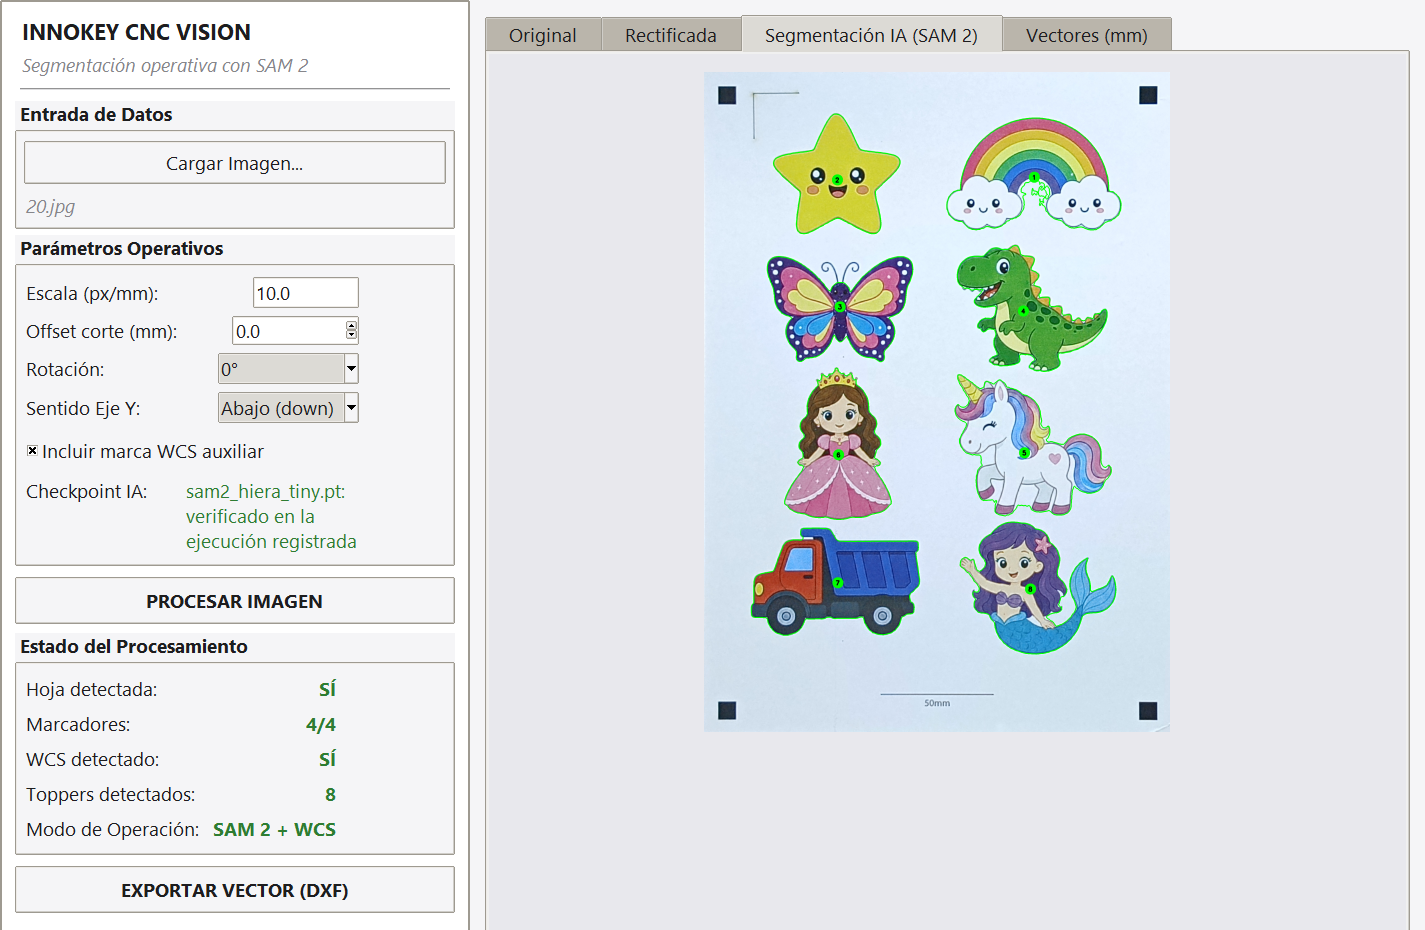
\includegraphics[width=0.90\linewidth]{figuras/interfaz_final/gui_final_03_sam2_document.png}
\captionof{figure}[Vista completa de la interfaz final.]{Vista completa de la interfaz tras procesar la captura 20 con SAM 2 y WCS.}
\label{fig:gui_sam2}
\end{landscape}

Para mantener legibles los controles y las pestañas, la ventana completa se presenta en formato apaisado en la Figura~\ref{fig:gui_sam2}. El detalle de la Figura~\ref{fig:gui_sam2_detalle} amplía los dos elementos que intervienen directamente en la decisión de exportar: el diagnóstico de la ejecución y la segmentación revisada por el usuario.

\figuraopcional{gui_sam2_legible}{0.92\textwidth}{Detalle ampliado del estado operativo y de la salida de SAM 2 en la captura 20.}{fig:gui_sam2_detalle}

La inspección no termina en la máscara. La pestaña vectorial representa en milímetros las ocho trayectorias exteriores y la referencia WCS que viajarán al DXF. La Figura~\ref{fig:gui_vectores} documenta esta segunda vista de la aplicación con una ampliación suficiente para revisar ejes, identificadores y capas.

\figuraopcional{gui_vectores_legible}{0.90\textwidth}{Previsualización vectorial de las ocho trayectorias exteriores y de la referencia WCS antes de utilizar el DXF en el flujo CAM.}{fig:gui_vectores}

\section{Verificación de la integración}

La integración se evaluó mediante 23 pruebas automatizadas y varias ejecuciones de extremo a extremo. Una parte del conjunto comprueba la configuración y los estados de la aplicación, incluidos el bloqueo de escala y las condiciones que habilitan la exportación. Otra recorre la geometría, desde la detección WCS en las trece capturas y el caso ambiguo con dos marcas en L hasta la selección del contorno exterior, los huecos opcionales, el offset y la reapertura del DXF. El contrato de inteligencia artificial se verifica aparte: el extractor debe recibir la máscara producida por SAM 2 y la ruta neuronal debe detenerse si falta el checkpoint, sin recurrir silenciosamente a la visión clásica.

En la captura 20, la herramienta detectó un WCS válido, generó ocho cajas, obtuvo ocho componentes con SAM 2 y extrajo ocho siluetas exteriores. Otra prueba controlada confirmó que el modo operativo descarta una perforación interna, aunque la función opcional puede conservarla cuando se solicita expresamente. El conjunto demuestra la continuidad del software y la coherencia estructural y geométrica interna del archivo. El comportamiento de esas trayectorias sobre el material deberá medirse en una campaña de corte.
